\chapter{Video Compression}
\section{Perception of motion}
Perception of motion: Human visual system is specifically sensitive to motion. Eyes follow motion automatically. Some distortions are not as percoivable as in image coding (would be if we froze frame). No good psycho-visual model avaivable. Vusal perception is limited to $<\SI{24}{\hertz}$. Asuccession of images will be perceived as continuous if frequency is sufficiely high. Cinema $24\SI{24}{\hertz}$, TV $\SI{25}{\hertz}$ or $\SI{50}{\hertz}$. We still nee to avoid aliasing (wheel effect). High-rendering frame-rates desired in computer games (needed due to absence of motion blur). Flicker can be perceived up to $>\SI{60}{\hertz}$ in particular in periphery. Issue addressed by $\SI{100}{\hertz}$ TV.
\section{Interlaced video format}
Two temporarlly shifted half images, increase of frequency $\SI{25}{\hertz}\to\SI{50}{\hertz}$. Reduction of spatial resolution. Full image representation: progressive.
\section{Why compress video?}
Raw HD TV signal $720p@\SI{50}{\hertz}$:
\begin{align*}
	&1280\cdot720\cdot50\cdot\SI{24}{\bits/\second}\\
	&\quad=\SI{1105920000}{\bits/\second}>\SI{1}{\gb/\second}
\end{align*}
Only $\SI{20}{\mb/\second}$ HDTV channel bandwdith requires compression of factor of $60$ ($\SI{0.4}{\bits/\pixel}$ on average)
\section{Lossy video compression}
Take advantage of redundancy. Spatial correlation between neighboring pixels. Temporal correlation between frames. Drop perceptuall unimportant details.
\begin{compactdesc}
	\item[\lp{Temporal Redundancy}] Take advantage of similarity between successive frames
	\item[\lp{Temporal processing}]\hfill\\
			Usually high frame rate: Significant temporal redundancy. Possible representations along temporal dimension:\hfill\\
		\begin{enumerate*}[label=\protect\circled{\arabic*},itemjoin=]
			\item Transform/subband methods: Good for textbook case of constant velocity uniform global motion. Inefficient for nonuniform motion, i.e. real-world motion. Requires large number of frame stores which leads to delay. (Memory cost may alse be an issue.) Is ineffective for many scene changes or high motion.\\
			\item Prodictive methods: Good performance using only 2 frame stores. However, simple frame differencing is not enough\ldots
		\end{enumerate*}
	\item[\lp{Goal}] Exploit the temporal redundancy
	\item[\lp{Predict current frame}] based on previously coded frames
	\item[\lp{Types of coded frames:}]\hfill\\
		\begin{enumerate*}[label=\protect\circled{\arabic*},itemjoin=]
			\item I-frame: Intra-coded frame, coded independently of all other frames.\\
			\item P-frame: Predictively coded frame, coded based on previously coded frame I or P. Can send motion vector plus changes.\\
			\item B-frame: Bi-directionally predicted frame, coded based on both previous and future coded frames I and P. In case something is uncovered.
		\end{enumerate*}
	\item[\lp{Motion-compensated prediction}] Simple frame differencing \emph{fails} when there is motion. Must account for motion. $\to$ Motion-compensated (MC) prediction. MC-prediction generally provides significant improvements. Questions: How can we estimate motion? How can we form MC-prediction?
	\item[\lp{Ideal situation}]\hfill\\
		\begin{enumerate*}[label=\protect\circled{\arabic*},itemjoin=]
			\item Partition video into moving objects \\
			\item describe object motion $\to$ Generally very difficult\\
		\end{enumerate*}
	\item[\lp{Practical approach}] Block-Matching Motion Estimation:\hfill\\
		\begin{enumerate*}[label=\protect\circled{\arabic*},itemjoin=]
			\item Partition each frame into blocks, e.g. $16\times\SI{16}{\pixels}$\\
			\item Describe motion of each block\\
		\end{enumerate*}
		$\to$  No object identification required and good, robust performance.
\section{Block-matching motion estimation}
\item[\lp{Assumptions:}]
\begin{enumerate*}[label=\protect\circled{\arabic*},itemjoin=]
	\item Translational motion within block:\\
		$f(n_1,n_2,k_{\text{cur}})$\\$\quad=f(n_1-mv_1,n_2-mv_2,k_{\text{ref}}).$
\end{enumerate*}
\item[\lp{ME Algorithm}] 
	\begin{enumerate*}[label=\protect\circled{\arabic*},itemjoin=]
		\item Divide current frame into non-overlapping $N_1\times N_2$ blocks.\\
		\item For each block, find the best matching block in reference frame.
	\end{enumerate*}
\subsection{Determining the best matching block}
For each block in the current frame, search for best matching block in the reference frame.
	\item[\lp{Metrics}] for determining ``best match'':
		\begin{align*}\dls 
			&\text{MSE}\\[-1em]
			&={\scriptstyle\sum\limits_{\mathclap{n_1,n_2\in\text{Block}}}^{}}\left[f(n_1,n_2,k_{\text{cur}})\right.\\[-1ex]
			&\left.-f(n_1-mv_1,n_2-mv_2,k_{\text{ref}})\right]^2.\\
			&\text{MAE}\\[-1em]
			&={\scriptstyle\sum\limits_{\mathclap{n_1,n_2\in\text{Block}}}^{}}\left|f(n_1,n_2,k_{\text{cur}})\right.\\[-1ex]
			&\left.-f(n_1-mv_1,n_2-mv_2,k_{\text{ref}})\right|.
		\end{align*}
	\item[\lp{Candidate blocks}] All blocks in, e.g. $\left( \pm 32,\pm 32 \right)$ pixel area
	\item[\lp{Strategies for searching}] candidate blocks for best match.\\
		\begin{enumerate*}[label=\protect\circled{\arabic*},itemjoin=]
			\item Full search: Examine all candidate blocks\\
			\item Partial (fast) search: Examine a carefully selected subset.
		\end{enumerate*}
	\item[\lp{Motion vector}] Estimate of motion for best matching block.
\section{Motion vector and motion vector field}
	\item[\lp{Motion vector}] Expresses the \emph{relative horizontal and vertical offsets} $(mv_1,mv_2)$, or motion, of a given block from one frame to another.
	\item[\lp{Motion vector field}] Collection of motion vectors for all the blocks in a frame.
	\item[\lp{Example of fast motion estimation search}]
\pgr{VisComp06b_VideoCompression}{65}{-2.0}{-1.75}{2.25}{1}
\item[\lp{Motion Vector Presision}]\hfill\\
\begin{itemize*}[label=\colorbullet]
	\item Motivation: Motion is not limited to integer-pixel offsets. However, video is only known at discrete pixel locations. To estimate sub-pixel motion, frames must be spatially interpolated.\\
	\item Fractional MVs are used to represent the sub-pixel motion.\\
	\item Improved performance (extra complexity is worthwhile)\\
	\item Half-pixel ME used in most standards: MPEG-1/2/4\\
	\item Why are half-pixel motion vectors better? They can capture half-pixel motion. Averaging effect (from spatial interpolation) reduces prediction error $\to$ Improved prediction. For noisy sequences, averaging effect reduces noise $\to$ Improved compression.
\end{itemize*}
\subsection{Practical Half-Pixel Motion Estimation Algorithm}
Half-pixel ME (coarse-fine) algorithm:
\begin{enumerate*}[label=\protect\circled{\arabic*},itemjoin=]
	\item Coarse step: Perform integer motion estimation on blocks; find best integer-pixel MV\\
	\item Fine step: Refine estimate to find best half-pixel MV\\
		\begin{enumerate*}[label=\protect\circled{\alph*},itemjoin=]
			\item Spatially interpolate the selected region in reference frame\\
			\item Compare current block to interpolated reference frame block.\\
			\item Choose the integer or half-pixel offset that provides best match
		\end{enumerate*}
\end{enumerate*}
Typically, bilinear interpolation is used for spatial interpolation
\section{Block Matching Algorithm}
\item[\lp{Issues}] Block size, search range, motion vector accuracy
\item[\lp{Estimate}] Done typically only from luminance
\item[\lp{Advantages}] 
	\begin{enumerate*}[label=\protect\circled{\arabic*},itemjoin=]
		\item Good, robust performance for compression. \\
		\item Resulting motion vector field is easy to represent (one MV per block) and useful for compression. \\
		\item Simple, periodic structure, easy VLSI implementations
	\end{enumerate*}
\item[\lp{Disadvantages}] \hfill\\
	\begin{enumerate*}[label=\protect\circled{\arabic*},itemjoin=]
		\item Assumes translational motion model $\to$ Breaks down for more complex motion.\\
		\item Ofter produces blocking artifacts (OK for coding with Block DCT)
	\end{enumerate*}
\item[\lp{Bidirectional MC prediction}]
	is uset to estimate a block in the current frame from a block in:\\
	\begin{enumerate*}[label=\protect\circled{\arabic*},itemjoin=]
		\item Previous frame\\
		\item Future frame\\
		\item Average of ablock from the previous frame and a block from the future frame\\
		\item Neither, i.e. code current block without prediction
	\end{enumerate*}\\
	\emph{Example}: Prediction with P- and B-frames\\
	\begin{enumerate*}[label=\protect\circled{\arabic*},itemjoin=]
		\item Motion compensated prediction: Predict the current frame based on reference frame(s) while compensating for the motion.\\
		\item Examples of block-based motion-compensated prediction (P-frame) and bi-directional prediction (B-frame).
	\end{enumerate*}
\section{Frame types}
Main addition over image compression: Exploit the temporal redundancy. Predict current frame based on previously coded frames. Three types of coded frames:\\
\begin{enumerate*}[label=\protect\circled{\arabic*},itemjoin=]
	\item \emph{I-frame}: Intra-coded frame, coded independently of all other frames\\
	\item \emph{P-frame}: Predictively coded frame, coded based on previously coded frame\\
	\item \emph{B-frame}: Bi-directionally predicted frame, coded based on both previous and future coded frames.\\
\end{enumerate*}
\item[\lp{MPEG Group of Pictures (GOP)}] \hfill
		\begin{center}
			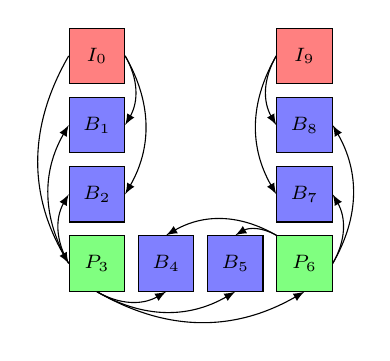
\begin{tikzpicture}
				\node[rectangle,draw,minimum width=2em,minimum height=2em,fill=red!50!white] (i0) at (0,0) {$\scriptstyle I_0$};
				\node[rectangle,draw,minimum width=2em,minimum height=2em,fill=blue!50!white] (b1) at (0,-2.5em) {$\scriptstyle B_1$};
				\node[rectangle,draw,minimum width=2em,minimum height=2em,fill=blue!50!white] (b2) at (0,-5em) {$\scriptstyle B_2$};
				\node[rectangle,draw,minimum width=2em,minimum height=2em,fill=green!50!white] (p3) at (0,-7.5em) {$\scriptstyle P_3$};
				\node[rectangle,draw,minimum width=2em,minimum height=2em,fill=blue!50!white] (b4) at (2.5em,-7.5em) {$\scriptstyle B_4$};
				\node[rectangle,draw,minimum width=2em,minimum height=2em,fill=blue!50!white] (b5) at (5em,-7.5em) {$\scriptstyle B_5$};
				\node[rectangle,draw,minimum width=2em,minimum height=2em,fill=green!50!white] (p6) at (7.5em,-7.5em) {$\scriptstyle P_6$};
				\node[rectangle,draw,minimum width=2em,minimum height=2em,fill=blue!50!white] (b7) at (7.5em,-5em) {$\scriptstyle B_7$};
				\node[rectangle,draw,minimum width=2em,minimum height=2em,fill=blue!50!white] (b8) at (7.5em,-2.5em) {$\scriptstyle B_8$};
				\node[rectangle,draw,minimum width=2em,minimum height=2em,fill=red!50!white] (i9) at (7.5em,-0em) {$\scriptstyle I_9$};
				\path[-latex,draw] (i0.west) to[bend right] node{} (p3.west);
				\path[-latex,draw] (i0.east) to[bend left] node{} (b1.east);
				\path[-latex,draw] (i0.east) to[bend left] node{} (b2.east);
				\path[-latex,draw] (p3.west) to[bend left] node{} (b1.west);
				\path[-latex,draw] (p3.west) to[bend left] node{} (b2.west);
				\path[-latex,draw] (p3.south) to[bend right] node{} (b4.south);
				\path[-latex,draw] (p3.south) to[bend right] node{} (b5.south);
				\path[-latex,draw] (p3.south) to[bend right] node{} (p6.south);
				\path[-latex,draw] (p6.east) to[bend right] node{} (b7.east);
				\path[-latex,draw] (p6.east) to[bend right] node{} (b8.east);
				\path[-latex,draw] (i9.west) to[bend right] node{} (b8.west);
				\path[-latex,draw] (i9.west) to[bend right] node{} (b7.west);
				\path[-latex,draw] (p6.north west) to[bend right] node{} (b4.north);
				\path[-latex,draw] (p6.north west) to[bend right] node{} (b5.north);
			\end{tikzpicture}
		\end{center}
		Starts with an I-frame, ends with frame right before next I-frame. ``Open'' ends in B-frame, ``closed'' in P-frame. MPEG Encoding a parameter, but ``typical'':
		\begin{align*}
			&IBBPBBPBBI,\\
			&IBBPBBPBBPBBI.
		\end{align*}
		Periodic I-frames enable random access into the coded bitstream. Parameters:\\
		\begin{enumerate*}[label=\protect\circled{\arabic*},itemjoin=]
			\item Spacing between I frames\\
			\item Number of B frames between I and P frames
		\end{enumerate*}
	\item[\lp{Example compression performance}] \hfill\\I: $\frac{1}{7}$, P: $\frac{1}{20}$, B: $\frac{1}{50}$, Average: $\frac{1}{27}$.
\section{Summary of Temporal Processing}
	\begin{enumerate*}[label=\protect\circled{\arabic*},itemjoin=]
		\item Use MC-prediction (P and P frames) to reduce temporal redundancy.\\
		\item MC-prediction usually performs well; In compression have a second changce to recover when it performs badly.\\
		\item MC-prediction yields\\
			\begin{enumerate*}[label=\quad\protect\circled{\alph*},itemjoin=]
				\item Motion vectors\\
				\item MC-prediction error or residual $\to$ Code error with conventional image coder\\
			\end{enumerate*}
		\item Sometimes MC-prediction may \emph{perform badly}\\
			\begin{enumerate*}[label=\quad\protect\circled{\alph*},itemjoin=]
				\item Examples: complex motion, new imagery (occlusions)\\
				\item Approach: \emph{1.} Identify frame or individual blocks where prediction fails \\
					\emph{2.} Code without prediction
			\end{enumerate*}
	\end{enumerate*}
	\section{Basic Video Compression Architecture}
	\begin{enumerate*}[label=\protect\circled{\arabic*},itemjoin=]
		\item Exploiting the reduncancies:\\
			\begin{enumerate*}[label=\quad\protect\circled{\alph*},itemjoin=]
				\item Temporal: MC-prediction (P and B frames)\\
				\item Spatial: Block DCT\\
				\item Color: color space conversion\\
			\end{enumerate*}
		\item Scalar quantization of DCT coefficients\\
		\item Zigzag scanning, runlength and Huffman coding of the nonzero quantized DCT coefficients
	\end{enumerate*}
	\pgrr{VisComp06b_VideoCompression}{83}{-2.6}{-1.9}{2.5}{1.1}{90}
	\pgrr{VisComp06b_VideoCompression}{84}{-2.6}{-1.65}{2.52}{0.9}{90}
	\pgrr{VisComp06b_VideoCompression}{85}{-2.6}{-1.65}{2.52}{1.0}{90}
	\pgrr{VisComp06b_VideoCompression}{86}{-2.6}{-1.65}{2.52}{1.0}{90}
\item[\lp{Transimission chain}] Content Creation $\to$ Transmission $\to$ Consumption. $\Rightarrow$ Variable needs!
\section{Scalable Video Coding}
Produces \emph{different layers with prioritized importance}. \emph{Prioritized importance is key} for a variety of applications:\\
\begin{enumerate*}[label=\protect\circled{\arabic*},itemjoin=]
	\item \emph{Adapting} to different bandwidths, or client resources such as spatial or temporal resolution or computational power.\\
	\item \emph{Facilililates error-resilience} by explicitly identifying most important and less important bits.\\
\end{enumerate*}
\emph{Procedure}:\\
\begin{enumerate*}[label=\protect\circled{\arabic*},itemjoin=]
	\item Decompose video into \emph{multiple layers of prioritized importance}\\
	\item Code layers into \emph{base and enhancement} bitstreams\\
	\item Progressively combine \emph{one or more bitstreams} to produce \emph{different levels of video quality}.\\
\end{enumerate*}
Example of scalable coding with base and two enhancement layers: Can produce three different qualities:
\begin{enumerate*}[label=\protect\circled{\arabic*}]
	\item Base layer
	\item Base + Enh1 layers
	\item Base + Enh1 + Enh2 layers
\end{enumerate*}
Scalability with respect to: Spatial or temporal resolution, bit rate, computation, memory.
\item[\lp{Example}]
	\begin{itemize*}[label=\colorbullet]
		\item Encode image/video into three layers: Base, Enh1, Enh2
		\item Low-bandwidth recoiver: Send only Base layer.
		\item Medium-bandwidth recoiver: Send Base \& Enh1 layers
		\item High-bandwidth receiver: Send all three layers Base, Enh1, Enh2.
		\item Can adapt to different clients and network situations
		\item Three basic types of scalability (refine video quality along three different dimensions):\\
			\begin{enumerate*}[label=\quad\protect\circled{\alph*},itemjoin=]
				\item Temporal scalability $\to$ Temporal resolution\\
				\item Spatial scalability $\to$ Spatial resolution\\
				\item SNR (quality) scalability $\to$ Amplitude resolution\\
			\end{enumerate*}
		\item Each type of scalable coding provides scalability of one dimension of the video signal. Can cambine multiple types of scalability to provide scalability along multiple dimensions
	\end{itemize*}
\item[\lp{Temporal Scalability}] based on the use of \emph{B-frames} to refine the \emph{temporal resolution} B-frames are dependent on other frames. Howere, no other frame depends on a B-frame. Each B-frame may be discarded without affecting other frames. 
\item[\lp{Spatial scalability}] Based on refining the \emph{spatial resolution} \emph{Base layer} is \emph{low resolution} version of video. \emph{Enh1} contains coded \emph{difference} between upsampled base layer and original video. Also called pyramid coding.
\item[\lp{SNR scalability}] Based on refining the \emph{amplitude resolution} \emph{Base layer} uses a \emph{coarse quantizer}. \emph{Enh1} applies a \emph{finer quantizer} to the difference between the original DCT coefficients and the coarsely quantized base layer coefficients.
\section{Standards}
	\item[\lp{Goal}] \emph{Ensuring interoperability}: Enbabling communication between devices made by different monufacturers. Promoting a technology or industry. Reducing costs.
	\item[\lp{Scope of standardization}] Not the encoder, not the decoder. Just the \emph{bitstream syntax} and the \emph{decoding process} (e.g. use IDCT but not how to implement the IDCT) This enables improved encoding and decoding strategies to be employed in a standard-compatible manner.
\section{Quality measure}
	\item[\lp{objective: PSNR}] \hfill\\
		\begin{itemize*}[label=\colorbullet]
			\item Error for one pixel, difference between original and decoded value\\
				$e(v,h)=\tilde{x}(v,h)-x(v,h)$\\
		\item Mean-squared-Error, MSE e.g. over an image\\
			$\ds e_{\text{MSE}}=\sqrt{\frac{1}{N\cdot M}{\scriptstyle\sum\limits_{v,h=1}^{\mathclap{\quad v=N,h=M}}}e^2(v,h)}$
		\item Peak-Signal-to-Noise-Ratio\\
			$\text{PSNR}=[\max x]^2/e_{\text{MSE}}^{2}$\\
			E.g. $x=2^K$ or $255$. One can use a $\log$-scale like $\si{\decibel}$.
		\end{itemize*}
	\item[\lp{MPEG Structure}] MPEG codes video in a \emph{hierarchy of layers}. The sequence layer is not shown.
	\item[\lp{MPEG-2}] \emph{Goal:} To enable more efficient implementations for different applications (interoperability points)\\
		\begin{itemize*}[label=\colorbullet]
			\item Profile: Subset of the tools applicable for a family of applications\\
			\item Level: bounds on the complexity for any profile
		\end{itemize*}
	\item[\lp{MPEG-4}] Natural Video Coding\\
		Extension of MPEG-1/2-type algorithms to code arbitrarily shaped objects.
	\item[\lp{Sprite Coding}] Background prediction. Hypothesis: Same background exists for many frames, changes resulting from camera motion and occlusions. One possible coding strategy:
		\begin{enumerate*}[label=\protect\circled{\arabic*},itemjoin=]
			\item Code \& transmit entire sprite \emph{once}\\
			\item Only transmit camera motion parameters for each subsequent frame
		\end{enumerate*}
		Significant coding gain for some scenes.
	\item[\lp{3D TV}] Requeires the transmission of multiple views (two or more). Opportunity to do better than simulateously broadcast multiple views. Besides intra-frame and temporal redundancy, also \emph{ex ploit inter-view redundancy}.
	\pgrr{VisComp06b_VideoCompression}{121}{-2.6}{-1.25}{2.52}{1.0}{90}
\end{compactdesc}
